\subsection{Dependency Injection}
Dependency injection\footnote{\url{http://en.wikipedia.org/wiki/Dependency_injection}} is a technique in software development that allows the developer to inject an implementation of an interface into a given module that depends on that interface. We use constructor injection meaning the dependency is given in the constructor call as seen in the example code-snippet in Figure \ref{fig:DependencyInjection}. Dependency injection hence allows for injecting different implementations of the same interface, e.g. into \texttt{EventStorage}.

\begin{figure}[h!]
\centering
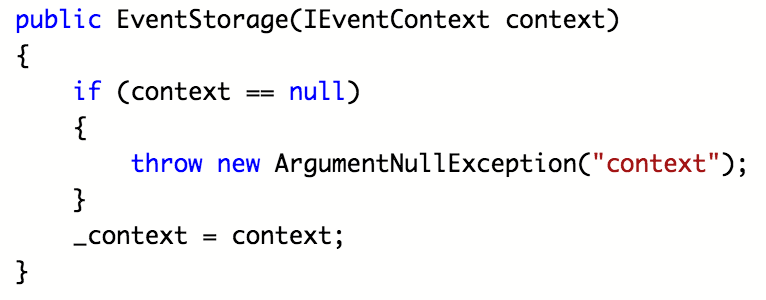
\includegraphics[width=0.7\linewidth]{figures/EventStorage1}
\caption{\label{fig:DependencyInjection}Here, in \texttt{EventStorage}, a context, implementing \texttt{IEventContext}, is passed to the constructor, that the \texttt{EventStorage} is to use.  }
\end{figure}

A major motivation for using dependency injection was not to inject different implementations during runtime, but instead for the team to mock dependencies when unit testing classes. The use of mocking is described in Section \ref{sec:UnitTesting} \nameref{sec:UnitTesting}.

Dependency injection is very useful for testing since it is possible to test a module in isolation by injecting mocked interfaces into the module being tested. An example of isolation is to not run storage tests against the actual database but instead against a mocked implementation of the database. 

This enabled testing in a controlled environment and allowed for more verifiable tests without side effects.